\subsection{Overview}
% \begin{algorithm}[t]
\small
% \caption{\textsc{$(r,s)$-CND}}
% \label{alg:framework}
% \KwIn{Clique size $s$}
% \KwOut{Core value $\kappa_s(v)$ for every vertex $v$}
% \SetKwFunction{RemoveNode}{RemoveNode}
% \SetKwFunction{CountPreEdges}{$s$-CliqueCount}
% \SetKwProg{Fn}{Function}{:}{}

% $\tree$ $\leftarrow$ build CPI of $G$, pruning paths with $s$\;

% $support \gets$ \textsc{CountPreEdges}$(\mathcal{B}, r, s)$\;

% build min heap $H_{\min}$ using $support$\;

% $c_{min} \gets 0$\;

% \While{$H_{\min}$ is not empty}{
%     $R_{min} \gets \text{ExtractMin}(H_{\min})$\;
%     $c_{min} \gets \max(c_{min}, support(R_{min}))$\;
%     $\kappa_s(R_{min}) \gets c_{min}$\;
%     \ForEach{leaf $\TPath$ intersecting any $rc \in R_{min}$}{
%         $B \gets {\,rc \in R_{min} \mid rc \in \TPath\,}$\;
%         \text{Remove all $r$-cliques in $B$ from $\TPath$}\;
%     }

%     \ForEach{leaf $\TPath$ containing any $rc \in R_{min}$}{
%         Update $support(rc)$ and $H_{\min}$ for all $r$-clique $rc \in \TPath$
%     }

% }

% \Return{$\kappa_s(r)$ for all $r$-cliques $r$ in $\tree$}\;

% \end{algorithm}

\begin{algorithm}[t]
\small
\caption{\textsc{$(r,s)$-\cbnd}}
\label{alg:framework}
\KwIn{Graph $G=(V,E)$, clique sizes $r<s$}
\KwOut{Core value $\kappa_s(R)$ for every $r$-clique $R$}
\SetKwFunction{RemoveNode}{RemoveNode}
\SetKwFunction{CountPreEdges}{$s$-CliqueCount}
\SetKwProg{Fn}{Function}{:}{}

$\tree \leftarrow \textsc{BuildIndex}(G)$\;

\tcp{initialize $s$-support for all $r$-cliques}

$support \gets$ \textsc{$s$-CliqueCount}$(\tree, r, s)$ 

build a min-heap $H_{\min}$ using $support$\;

$c_{min} \gets 0$\;

\While{$H_{\min}$ is not empty}{
    $R_{min} \gets \text{ExtractMin}(H_{\min})$\;
    $c_{min} \gets \max(c_{min}, support(R_{min}))$\;
    $\kappa_s(R_{min}) \gets c_{min}$\;
    
    % remove $R_{min}$ from index
    % Remove all $r$-cliques in $R_{min}$ from $\tree$\;
    \textsc{UpdateIndex}($R_{min}$, $\tree$) \tcp*{remove $R_{min}$ from $\tree$}

    \tcp{update support of affected $r$-cliques}

    \textsc{UpdateSupport}($R_{min}$, $\tree$, $support$, $H_{\min}$)

}

\Return{$\kappa_s(R)$ for all $r$-cliques $R$ in $\tree$}\;

\end{algorithm}

% 我们观察到, Nuclear Decomposition这个算法的输出只涉及到r-clique的coreness, 以及后续的hierarchy, 这些输出并不需要列举任何s-clique. s-clique仅仅是用来衡量r-clique的support, 因此我们认为避免显式的枚举s-clique是可行的. 
We observe that a key step in nucleus core decomposition is support computation.
%
For each $r$-clique, this step only needs the number of $s$-cliques that contain it.
%
This suggests that explicit enumeration of $s$-cliques is not necessary.
%
It is both feasible and desirable to avoid it.
Based on this observation, we propose a minimal counting-and-indexing layer, as shown in Algorithm~\ref{alg:framework}.



% 受此启发, 我们提出了一个最小化的基础框架, 如算法\ref{alg:framework}所示.
% 这个框架的关键在于通过索引来避免显式枚举s-clique, 具体来说有三个关键的操作需要索引来支持, 分别是: (i) 初始化每个r-clique的s-support(第2行), (ii) 删除已经peel掉的r-clique(第9行), 以及(iii) 精准识别和更新剩余受影响r-clique的support(第10行).
\stitle{Key Idea.} 
The core idea is simple.
%
We avoid explicit enumeration of $s$-cliques by using an auxiliary index. 
%
Our method still follows the peeling paradigm.
%
The index supports four key operations:
%
(i) \textsc{BuildIndex}, which initializes the auxiliary index structure (Line~1);  
(ii) \textsc{$s$-CliqueCount}, which computes the initial $s$-support for each $r$-clique (Line~2);  
(iii) \textsc{UpdateIndex}, which removes peeled $r$-cliques from the index (Line~9); and  
(iv) \textsc{UpdateSupport}, which identifies and updates the supports of affected $r$-cliques after each removal (Line~10).  
%
In the conference version, these four operations were mainly presented from a counting/indexing viewpoint.
%
In this journal version, operations (iii) and (iv) are lifted to the \emph{differential path contribution maintenance} view.
%
\textsc{UpdateIndex} only changes the local state of affected paths.
%
\textsc{UpdateSupport} uses exact differential updates of path contributions.
%
It does not use reconstructive support recomputation.
% 
\myaddRC{
Figure~\ref{fig:pipline} illustrates the overall pipeline of our approach.
}

\myaddRC{
\begin{figure}[t]
    \centering
    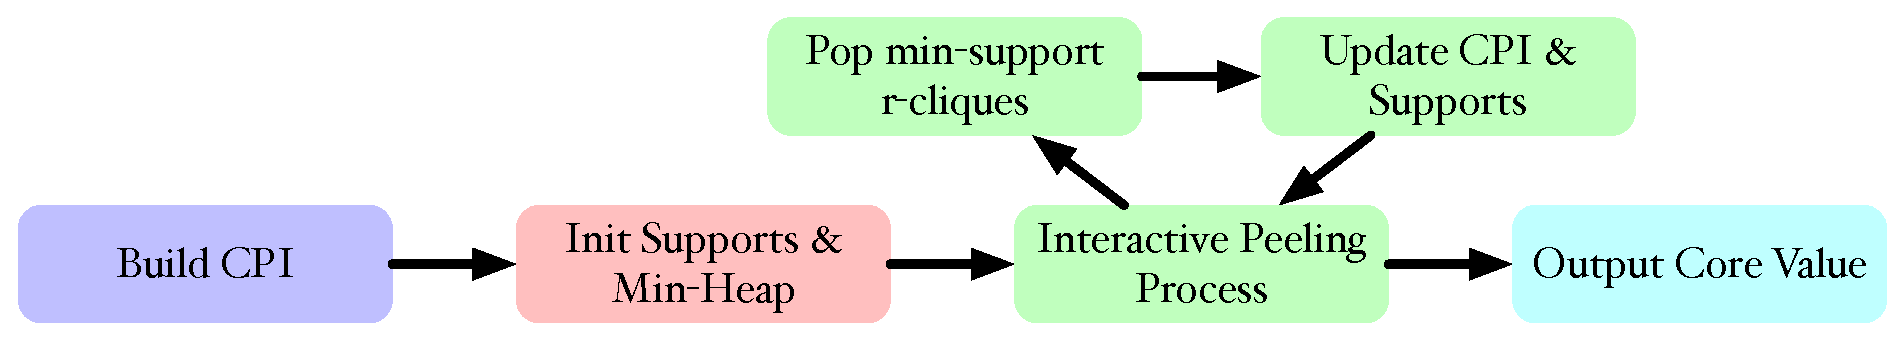
\includegraphics[width=0.45\textwidth]{figure/pipline.eps}
    % 虚线连接的节点是\pivot节点, 实线连接的节点是\hold节点.
    \caption{
        Overview of our approach.
    }
    \label{fig:pipline}
\end{figure}
}


\stitle{Index Support.}
% 上面说了4个
If an index supports these four operations efficiently, then nucleus decomposition can be performed without enumerating any $s$-cliques.
%
This removes the main bottleneck.
%
The key journal-level refinement is also simple.
%
The index is not only a compact representation of clique space.
%
It also carries the differential maintenance state used for exact support updates.
% 如果我们能找到一个索引来支持这三个操作, 那么我们就能在不枚举任何s-clique的情况下完成nuclear decomposition, 从而使算法变得不依赖于s-clique的枚举, 彻底摆脱枚举的瓶颈.


% Guided by this, we propose a minimal base framework: (i) build a CPI over $G$; (ii) compute the initial $s$-support for every $r$-clique; and (iii) peel in increasing support by repeatedly extracting the current minimum, assigning $\kappa_s(\cdot)$, removing the peeled $r$-cliques from CPI, and updating the supports of remaining neighbors along affected paths.

% To realize this framework \emph{without materializing $K_s$}, three lines in Algorithm~\ref{alg:hierarchy} require an index: line~2 (one-shot support initialization), line~11 (path-local removal of peeled $r$-cliques), and line~13 (incremental neighbor updates). Our goal is to carry out all three by \emph{counting} on CPI paths rather than \emph{enumerating} $s$-cliques.
